\documentclass{standalone}
\usepackage{tikz}
\usetikzlibrary{patterns, positioning}
\usepackage[sfdefault]{ClearSans} %% option 'sfdefault' activates Clear Sans as the default text font
\usepackage[T1]{fontenc}

\begin{document}
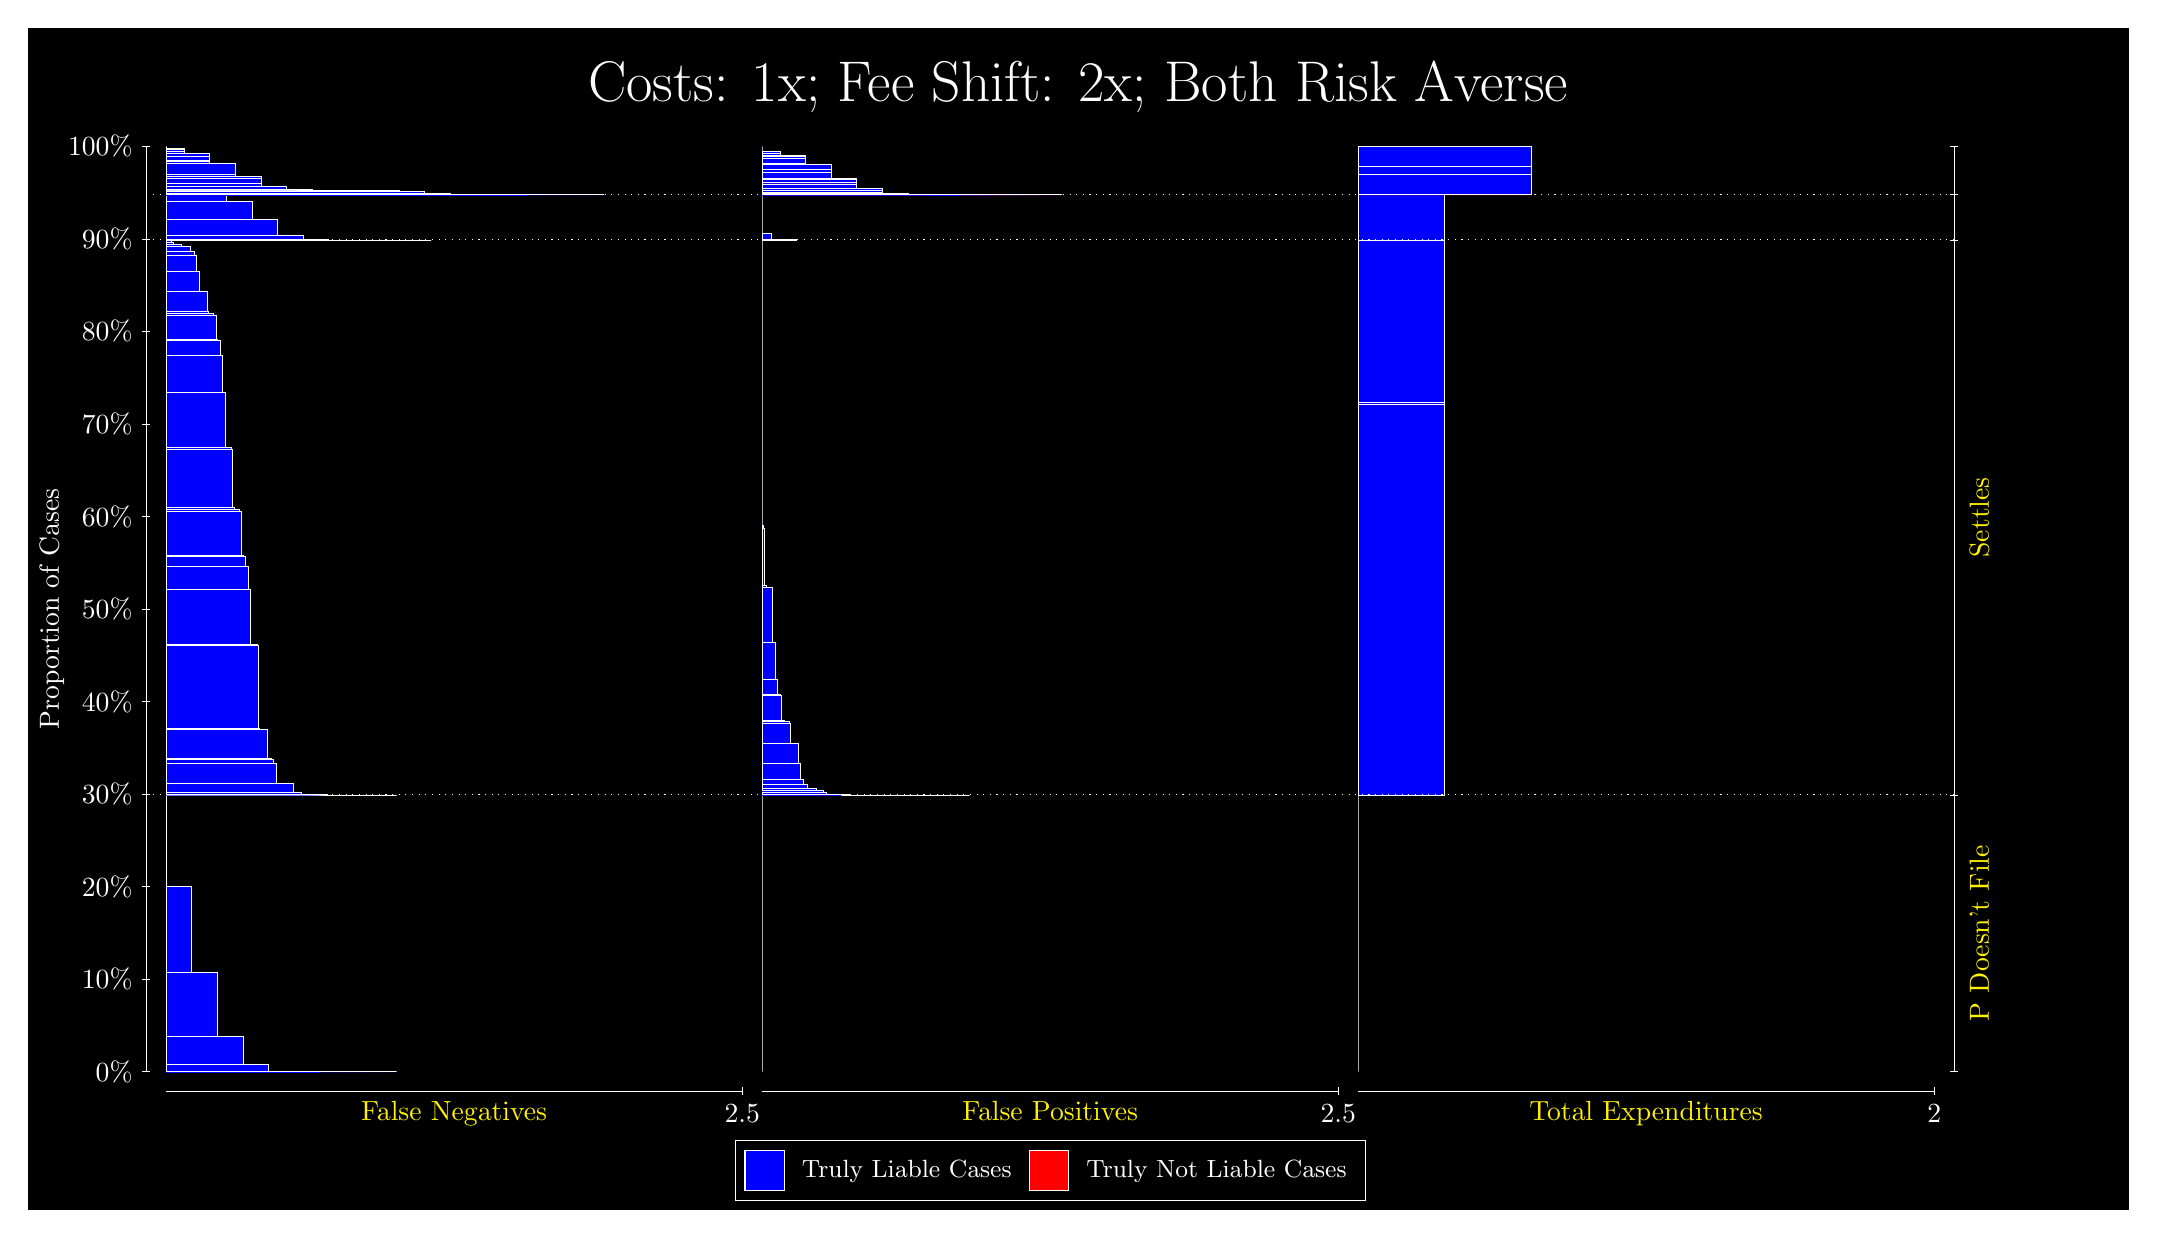
\begin{tikzpicture}
\draw[fill=black] (0,0) rectangle (26.667,15);
\draw[text=white] (0,13.5) rectangle (26.667,15) node[midway] {\huge Costs: 1x; Fee Shift: 2x; Both Risk Averse};
\draw[white, very thin] (1.5,1.75) -- (1.5,13.5);
\node[rotate=90, text=white, anchor=center] at (0.3, 7.625) {Proportion of Cases};
\draw[white, very thin] (1.45,1.75) -- (1.55,1.75);
\node[text=white, anchor=east] at (1.45, 1.75) {0\%};
\draw[white, very thin] (1.45,2.925) -- (1.55,2.925);
\node[text=white, anchor=east] at (1.45, 2.925) {10\%};
\draw[white, very thin] (1.45,4.1) -- (1.55,4.1);
\node[text=white, anchor=east] at (1.45, 4.1) {20\%};
\draw[white, very thin] (1.45,5.275) -- (1.55,5.275);
\node[text=white, anchor=east] at (1.45, 5.275) {30\%};
\draw[white, very thin] (1.45,6.45) -- (1.55,6.45);
\node[text=white, anchor=east] at (1.45, 6.45) {40\%};
\draw[white, very thin] (1.45,7.625) -- (1.55,7.625);
\node[text=white, anchor=east] at (1.45, 7.625) {50\%};
\draw[white, very thin] (1.45,8.8) -- (1.55,8.8);
\node[text=white, anchor=east] at (1.45, 8.8) {60\%};
\draw[white, very thin] (1.45,9.975) -- (1.55,9.975);
\node[text=white, anchor=east] at (1.45, 9.975) {70\%};
\draw[white, very thin] (1.45,11.15) -- (1.55,11.15);
\node[text=white, anchor=east] at (1.45, 11.15) {80\%};
\draw[white, very thin] (1.45,12.325) -- (1.55,12.325);
\node[text=white, anchor=east] at (1.45, 12.325) {90\%};
\draw[white, very thin] (1.45,13.5) -- (1.55,13.5);
\node[text=white, anchor=east] at (1.45, 13.5) {100\%};

\draw[white, very thin] (24.457,1.75) -- (24.457,13.5);
\draw[white, very thin] (24.407,1.75) -- (24.507,1.75);
\node[anchor=west] at (24.407, 1.75) {};
\draw[white, very thin] (24.407,5.264) -- (24.507,5.264);
\node[anchor=west] at (24.407, 5.264) {};
\draw[white, very thin] (24.407,12.311) -- (24.507,12.311);
\node[anchor=west] at (24.407, 12.311) {};
\draw[white, very thin] (24.407,12.885) -- (24.507,12.885);
\node[anchor=west] at (24.407, 12.885) {};
\draw[white, very thin] (24.407,13.5) -- (24.507,13.5);
\node[anchor=west] at (24.407, 13.5) {};

\draw[white, very thin, fill=blue] (1.75,1.75) rectangle (4.6775,1.75);
\draw[white, very thin, fill=blue] (1.75,1.75) rectangle (4.3523,1.75);
\draw[white, very thin, fill=blue] (1.75,1.75) rectangle (4.027,1.75);
\draw[white, very thin, fill=blue] (1.75,1.75) rectangle (3.7017,1.7503);
\draw[white, very thin, fill=blue] (1.75,1.7503) rectangle (3.3764,1.7576);
\draw[white, very thin, fill=blue] (1.75,1.7576) rectangle (3.0511,1.8361);
\draw[white, very thin, fill=blue] (1.75,1.8361) rectangle (2.7258,2.1984);
\draw[white, very thin, fill=blue] (1.75,2.1984) rectangle (2.4006,3.0086);
\draw[white, very thin, fill=blue] (1.75,3.0086) rectangle (2.0753,4.0995);
\draw[white, very thin, fill=red] (1.75,4.0995) rectangle (1.75,4.0995);
\draw[white, very thin, fill=blue] (1.75,4.0995) rectangle (1.75,5.264);
\draw[white, very thin, fill=blue] (1.75,5.264) rectangle (4.6775,5.264);
\draw[white, very thin, fill=blue] (1.75,5.264) rectangle (4.5312,5.264);
\draw[white, very thin, fill=blue] (1.75,5.264) rectangle (4.3848,5.264);
\draw[white, very thin, fill=blue] (1.75,5.264) rectangle (4.3523,5.264);
\draw[white, very thin, fill=blue] (1.75,5.264) rectangle (4.2384,5.264);
\draw[white, very thin, fill=blue] (1.75,5.264) rectangle (4.2059,5.264);
\draw[white, very thin, fill=blue] (1.75,5.264) rectangle (4.092,5.264);
\draw[white, very thin, fill=blue] (1.75,5.264) rectangle (4.0595,5.264);
\draw[white, very thin, fill=blue] (1.75,5.264) rectangle (4.027,5.264);
\draw[white, very thin, fill=blue] (1.75,5.264) rectangle (3.9131,5.264);
\draw[white, very thin, fill=blue] (1.75,5.264) rectangle (3.8806,5.264);
\draw[white, very thin, fill=blue] (1.75,5.264) rectangle (3.7993,5.265);
\draw[white, very thin, fill=blue] (1.75,5.265) rectangle (3.7668,5.265);
\draw[white, very thin, fill=blue] (1.75,5.265) rectangle (3.7342,5.265);
\draw[white, very thin, fill=blue] (1.75,5.265) rectangle (3.7017,5.265);
\draw[white, very thin, fill=blue] (1.75,5.265) rectangle (3.6529,5.265);
\draw[white, very thin, fill=blue] (1.75,5.265) rectangle (3.5878,5.265);
\draw[white, very thin, fill=blue] (1.75,5.265) rectangle (3.5553,5.265);
\draw[white, very thin, fill=blue] (1.75,5.265) rectangle (3.474,5.2928);
\draw[white, very thin, fill=blue] (1.75,5.2928) rectangle (3.4415,5.2951);
\draw[white, very thin, fill=blue] (1.75,5.2951) rectangle (3.4089,5.2954);
\draw[white, very thin, fill=blue] (1.75,5.2954) rectangle (3.3764,5.2956);
\draw[white, very thin, fill=blue] (1.75,5.2956) rectangle (3.3602,5.4081);
\draw[white, very thin, fill=blue] (1.75,5.4081) rectangle (3.3276,5.4084);
\draw[white, very thin, fill=blue] (1.75,5.4084) rectangle (3.2626,5.4092);
\draw[white, very thin, fill=blue] (1.75,5.4092) rectangle (3.23,5.4098);
\draw[white, very thin, fill=blue] (1.75,5.4098) rectangle (3.1487,5.6612);
\draw[white, very thin, fill=blue] (1.75,5.6612) rectangle (3.1162,5.714);
\draw[white, very thin, fill=blue] (1.75,5.714) rectangle (3.0837,5.7301);
\draw[white, very thin, fill=blue] (1.75,5.7301) rectangle (3.0511,5.7336);
\draw[white, very thin, fill=blue] (1.75,5.7336) rectangle (3.0349,6.094);
\draw[white, very thin, fill=blue] (1.75,6.094) rectangle (3.0023,6.099);
\draw[white, very thin, fill=blue] (1.75,6.099) rectangle (2.9373,6.1096);
\draw[white, very thin, fill=blue] (1.75,6.1096) rectangle (2.921,7.1616);
\draw[white, very thin, fill=blue] (1.75,7.1616) rectangle (2.9048,7.1707);
\draw[white, very thin, fill=blue] (1.75,7.1707) rectangle (2.8234,7.869);
\draw[white, very thin, fill=blue] (1.75,7.869) rectangle (2.7909,8.1662);
\draw[white, very thin, fill=blue] (1.75,8.1662) rectangle (2.7584,8.2942);
\draw[white, very thin, fill=blue] (1.75,8.2942) rectangle (2.7258,8.3063);
\draw[white, very thin, fill=blue] (1.75,8.3063) rectangle (2.7096,8.865);
\draw[white, very thin, fill=blue] (1.75,8.865) rectangle (2.6771,8.8887);
\draw[white, very thin, fill=blue] (1.75,8.8887) rectangle (2.612,8.9222);
\draw[white, very thin, fill=blue] (1.75,8.9222) rectangle (2.5957,9.6524);
\draw[white, very thin, fill=blue] (1.75,9.6524) rectangle (2.5795,9.6753);
\draw[white, very thin, fill=blue] (1.75,9.6753) rectangle (2.4982,10.374);
\draw[white, very thin, fill=blue] (1.75,10.374) rectangle (2.4656,10.843);
\draw[white, very thin, fill=blue] (1.75,10.843) rectangle (2.4331,11.038);
\draw[white, very thin, fill=blue] (1.75,11.038) rectangle (2.4006,11.046);
\draw[white, very thin, fill=blue] (1.75,11.046) rectangle (2.3843,11.36);
\draw[white, very thin, fill=blue] (1.75,11.36) rectangle (2.3518,11.383);
\draw[white, very thin, fill=blue] (1.75,11.383) rectangle (2.2867,11.407);
\draw[white, very thin, fill=blue] (1.75,11.407) rectangle (2.2705,11.653);
\draw[white, very thin, fill=blue] (1.75,11.653) rectangle (2.2542,11.662);
\draw[white, very thin, fill=blue] (1.75,11.662) rectangle (2.1729,11.911);
\draw[white, very thin, fill=blue] (1.75,11.911) rectangle (2.1403,12.113);
\draw[white, very thin, fill=blue] (1.75,12.113) rectangle (2.1078,12.171);
\draw[white, very thin, fill=blue] (1.75,12.171) rectangle (2.0753,12.173);
\draw[white, very thin, fill=blue] (1.75,12.173) rectangle (2.059,12.226);
\draw[white, very thin, fill=blue] (1.75,12.226) rectangle (2.0265,12.231);
\draw[white, very thin, fill=blue] (1.75,12.231) rectangle (1.9614,12.234);
\draw[white, very thin, fill=blue] (1.75,12.234) rectangle (1.9452,12.258);
\draw[white, very thin, fill=blue] (1.75,12.258) rectangle (1.9289,12.259);
\draw[white, very thin, fill=blue] (1.75,12.259) rectangle (1.8476,12.283);
\draw[white, very thin, fill=blue] (1.75,12.283) rectangle (1.8151,12.304);
\draw[white, very thin, fill=blue] (1.75,12.304) rectangle (1.7825,12.307);
\draw[white, very thin, fill=red] (1.75,12.307) rectangle (1.75,12.307);
\draw[white, very thin, fill=blue] (1.75,12.307) rectangle (1.75,12.311);
\draw[white, very thin, fill=blue] (1.75,12.311) rectangle (5.1167,12.311);
\draw[white, very thin, fill=blue] (1.75,12.311) rectangle (4.7914,12.311);
\draw[white, very thin, fill=blue] (1.75,12.311) rectangle (4.4661,12.311);
\draw[white, very thin, fill=blue] (1.75,12.311) rectangle (4.1408,12.311);
\draw[white, very thin, fill=blue] (1.75,12.311) rectangle (3.8155,12.315);
\draw[white, very thin, fill=blue] (1.75,12.315) rectangle (3.4903,12.367);
\draw[white, very thin, fill=blue] (1.75,12.367) rectangle (3.165,12.576);
\draw[white, very thin, fill=blue] (1.75,12.576) rectangle (2.8397,12.802);
\draw[white, very thin, fill=blue] (1.75,12.802) rectangle (2.5144,12.875);
\draw[white, very thin, fill=blue] (1.75,12.875) rectangle (2.1891,12.885);
\draw[white, very thin, fill=red] (1.75,12.885) rectangle (1.75,12.885);
\draw[white, very thin, fill=blue] (1.75,12.885) rectangle (7.3123,12.885);
\draw[white, very thin, fill=blue] (1.75,12.885) rectangle (6.9871,12.885);
\draw[white, very thin, fill=blue] (1.75,12.885) rectangle (6.6618,12.885);
\draw[white, very thin, fill=blue] (1.75,12.885) rectangle (6.3365,12.885);
\draw[white, very thin, fill=blue] (1.75,12.885) rectangle (6.3365,12.886);
\draw[white, very thin, fill=blue] (1.75,12.886) rectangle (6.0112,12.886);
\draw[white, very thin, fill=blue] (1.75,12.886) rectangle (6.0112,12.886);
\draw[white, very thin, fill=blue] (1.75,12.886) rectangle (5.6859,12.887);
\draw[white, very thin, fill=blue] (1.75,12.887) rectangle (5.6859,12.89);
\draw[white, very thin, fill=blue] (1.75,12.89) rectangle (5.3606,12.898);
\draw[white, very thin, fill=blue] (1.75,12.898) rectangle (5.3606,12.907);
\draw[white, very thin, fill=blue] (1.75,12.907) rectangle (5.2305,12.907);
\draw[white, very thin, fill=blue] (1.75,12.907) rectangle (5.0354,12.926);
\draw[white, very thin, fill=blue] (1.75,12.926) rectangle (5.0354,12.933);
\draw[white, very thin, fill=blue] (1.75,12.933) rectangle (4.9052,12.933);
\draw[white, very thin, fill=blue] (1.75,12.933) rectangle (4.7101,12.942);
\draw[white, very thin, fill=blue] (1.75,12.942) rectangle (4.58,12.942);
\draw[white, very thin, fill=blue] (1.75,12.942) rectangle (4.58,12.942);
\draw[white, very thin, fill=blue] (1.75,12.942) rectangle (4.3848,12.943);
\draw[white, very thin, fill=blue] (1.75,12.943) rectangle (4.2547,12.943);
\draw[white, very thin, fill=blue] (1.75,12.943) rectangle (4.2547,12.943);
\draw[white, very thin, fill=blue] (1.75,12.943) rectangle (4.0595,12.943);
\draw[white, very thin, fill=blue] (1.75,12.943) rectangle (4.0595,12.943);
\draw[white, very thin, fill=blue] (1.75,12.943) rectangle (3.9294,12.943);
\draw[white, very thin, fill=blue] (1.75,12.943) rectangle (3.7342,12.943);
\draw[white, very thin, fill=blue] (1.75,12.943) rectangle (3.7342,12.943);
\draw[white, very thin, fill=blue] (1.75,12.943) rectangle (3.6041,12.949);
\draw[white, very thin, fill=blue] (1.75,12.949) rectangle (3.4089,12.949);
\draw[white, very thin, fill=blue] (1.75,12.949) rectangle (3.2788,12.955);
\draw[white, very thin, fill=blue] (1.75,12.955) rectangle (3.2788,12.993);
\draw[white, very thin, fill=blue] (1.75,12.993) rectangle (3.0837,12.993);
\draw[white, very thin, fill=blue] (1.75,12.993) rectangle (2.9535,12.996);
\draw[white, very thin, fill=blue] (1.75,12.996) rectangle (2.9535,13.033);
\draw[white, very thin, fill=blue] (1.75,13.033) rectangle (2.9535,13.092);
\draw[white, very thin, fill=blue] (1.75,13.092) rectangle (2.9535,13.119);
\draw[white, very thin, fill=blue] (1.75,13.119) rectangle (2.6283,13.14);
\draw[white, very thin, fill=blue] (1.75,13.14) rectangle (2.6283,13.286);
\draw[white, very thin, fill=blue] (1.75,13.286) rectangle (2.303,13.31);
\draw[white, very thin, fill=blue] (1.75,13.31) rectangle (2.303,13.324);
\draw[white, very thin, fill=blue] (1.75,13.324) rectangle (2.303,13.374);
\draw[white, very thin, fill=blue] (1.75,13.374) rectangle (2.303,13.418);
\draw[white, very thin, fill=blue] (1.75,13.418) rectangle (1.9777,13.437);
\draw[white, very thin, fill=blue] (1.75,13.437) rectangle (1.9777,13.466);
\draw[white, very thin, fill=blue] (1.75,13.466) rectangle (1.9777,13.48);
\draw[white, very thin, fill=red] (1.75,13.48) rectangle (1.75,13.48);
\draw[white, very thin, fill=blue] (1.75,13.48) rectangle (1.75,13.5);
\draw[white, very thin, fill=red] (9.3189,1.75) rectangle (9.3189,1.75);
\draw[white, very thin, fill=blue] (9.3189,1.75) rectangle (9.3189,5.264);
\draw[white, very thin, fill=red] (9.3189,5.264) rectangle (11.954,5.264);
\draw[white, very thin, fill=blue] (9.3189,5.264) rectangle (11.954,5.264);
\draw[white, very thin, fill=blue] (9.3189,5.264) rectangle (11.628,5.264);
\draw[white, very thin, fill=red] (9.3189,5.264) rectangle (11.515,5.264);
\draw[white, very thin, fill=blue] (9.3189,5.264) rectangle (11.515,5.264);
\draw[white, very thin, fill=blue] (9.3189,5.264) rectangle (11.303,5.264);
\draw[white, very thin, fill=red] (9.3189,5.264) rectangle (11.222,5.264);
\draw[white, very thin, fill=blue] (9.3189,5.264) rectangle (11.222,5.264);
\draw[white, very thin, fill=blue] (9.3189,5.264) rectangle (11.189,5.264);
\draw[white, very thin, fill=red] (9.3189,5.264) rectangle (11.075,5.264);
\draw[white, very thin, fill=blue] (9.3189,5.264) rectangle (11.075,5.264);
\draw[white, very thin, fill=blue] (9.3189,5.264) rectangle (10.978,5.264);
\draw[white, very thin, fill=blue] (9.3189,5.264) rectangle (10.896,5.264);
\draw[white, very thin, fill=blue] (9.3189,5.264) rectangle (10.864,5.264);
\draw[white, very thin, fill=red] (9.3189,5.264) rectangle (10.783,5.264);
\draw[white, very thin, fill=blue] (9.3189,5.264) rectangle (10.783,5.264);
\draw[white, very thin, fill=blue] (9.3189,5.264) rectangle (10.75,5.264);
\draw[white, very thin, fill=blue] (9.3189,5.264) rectangle (10.653,5.264);
\draw[white, very thin, fill=red] (9.3189,5.264) rectangle (10.636,5.264);
\draw[white, very thin, fill=blue] (9.3189,5.264) rectangle (10.636,5.264);
\draw[white, very thin, fill=blue] (9.3189,5.264) rectangle (10.571,5.264);
\draw[white, very thin, fill=blue] (9.3189,5.264) rectangle (10.539,5.264);
\draw[white, very thin, fill=red] (9.3189,5.264) rectangle (10.49,5.264);
\draw[white, very thin, fill=blue] (9.3189,5.264) rectangle (10.49,5.264);
\draw[white, very thin, fill=blue] (9.3189,5.264) rectangle (10.457,5.2645);
\draw[white, very thin, fill=blue] (9.3189,5.2645) rectangle (10.425,5.265);
\draw[white, very thin, fill=red] (9.3189,5.265) rectangle (10.344,5.265);
\draw[white, very thin, fill=blue] (9.3189,5.265) rectangle (10.344,5.265);
\draw[white, very thin, fill=blue] (9.3189,5.265) rectangle (10.327,5.2655);
\draw[white, very thin, fill=blue] (9.3189,5.2655) rectangle (10.311,5.2656);
\draw[white, very thin, fill=blue] (9.3189,5.2656) rectangle (10.246,5.2657);
\draw[white, very thin, fill=blue] (9.3189,5.2657) rectangle (10.213,5.268);
\draw[white, very thin, fill=red] (9.3189,5.268) rectangle (10.197,5.268);
\draw[white, very thin, fill=blue] (9.3189,5.268) rectangle (10.197,5.268);
\draw[white, very thin, fill=blue] (9.3189,5.268) rectangle (10.165,5.2716);
\draw[white, very thin, fill=blue] (9.3189,5.2716) rectangle (10.132,5.2923);
\draw[white, very thin, fill=blue] (9.3189,5.2923) rectangle (10.1,5.3165);
\draw[white, very thin, fill=blue] (9.3189,5.3165) rectangle (10.018,5.3172);
\draw[white, very thin, fill=blue] (9.3189,5.3172) rectangle (10.002,5.3413);
\draw[white, very thin, fill=blue] (9.3189,5.3413) rectangle (9.9857,5.3446);
\draw[white, very thin, fill=blue] (9.3189,5.3446) rectangle (9.9206,5.3489);
\draw[white, very thin, fill=blue] (9.3189,5.3489) rectangle (9.8881,5.4027);
\draw[white, very thin, fill=blue] (9.3189,5.4027) rectangle (9.8718,5.4039);
\draw[white, very thin, fill=blue] (9.3189,5.4039) rectangle (9.8393,5.4619);
\draw[white, very thin, fill=blue] (9.3189,5.4619) rectangle (9.8068,5.6644);
\draw[white, very thin, fill=blue] (9.3189,5.6644) rectangle (9.7743,5.9129);
\draw[white, very thin, fill=blue] (9.3189,5.9129) rectangle (9.6929,5.9222);
\draw[white, very thin, fill=blue] (9.3189,5.9222) rectangle (9.6767,6.1687);
\draw[white, very thin, fill=blue] (9.3189,6.1687) rectangle (9.6604,6.1925);
\draw[white, very thin, fill=blue] (9.3189,6.1925) rectangle (9.5954,6.2154);
\draw[white, very thin, fill=blue] (9.3189,6.2154) rectangle (9.5628,6.5294);
\draw[white, very thin, fill=blue] (9.3189,6.5294) rectangle (9.5466,6.5376);
\draw[white, very thin, fill=blue] (9.3189,6.5376) rectangle (9.514,6.7321);
\draw[white, very thin, fill=blue] (9.3189,6.7321) rectangle (9.4815,7.2016);
\draw[white, very thin, fill=blue] (9.3189,7.2016) rectangle (9.449,7.9);
\draw[white, very thin, fill=blue] (9.3189,7.9) rectangle (9.3677,7.9229);
\draw[white, very thin, fill=blue] (9.3189,7.9229) rectangle (9.3514,8.6532);
\draw[white, very thin, fill=blue] (9.3189,8.6532) rectangle (9.3351,8.6866);
\draw[white, very thin, fill=blue] (9.3189,8.6866) rectangle (9.3189,12.311);
\draw[white, very thin, fill=red] (9.3189,12.311) rectangle (9.758,12.311);
\draw[white, very thin, fill=blue] (9.3189,12.311) rectangle (9.758,12.322);
\draw[white, very thin, fill=blue] (9.3189,12.322) rectangle (9.4327,12.395);
\draw[white, very thin, fill=blue] (9.3189,12.395) rectangle (9.3189,12.885);
\draw[white, very thin, fill=red] (9.3189,12.885) rectangle (13.125,12.885);
\draw[white, very thin, fill=blue] (9.3189,12.885) rectangle (13.125,12.885);
\draw[white, very thin, fill=red] (9.3189,12.885) rectangle (12.799,12.885);
\draw[white, very thin, fill=blue] (9.3189,12.885) rectangle (12.799,12.885);
\draw[white, very thin, fill=blue] (9.3189,12.885) rectangle (12.474,12.885);
\draw[white, very thin, fill=red] (9.3189,12.885) rectangle (12.474,12.885);
\draw[white, very thin, fill=blue] (9.3189,12.885) rectangle (12.474,12.885);
\draw[white, very thin, fill=blue] (9.3189,12.885) rectangle (12.149,12.885);
\draw[white, very thin, fill=blue] (9.3189,12.885) rectangle (12.149,12.885);
\draw[white, very thin, fill=red] (9.3189,12.885) rectangle (12.149,12.885);
\draw[white, very thin, fill=blue] (9.3189,12.885) rectangle (12.149,12.885);
\draw[white, very thin, fill=red] (9.3189,12.885) rectangle (11.824,12.885);
\draw[white, very thin, fill=blue] (9.3189,12.885) rectangle (11.824,12.886);
\draw[white, very thin, fill=blue] (9.3189,12.886) rectangle (11.824,12.886);
\draw[white, very thin, fill=blue] (9.3189,12.886) rectangle (11.824,12.886);
\draw[white, very thin, fill=red] (9.3189,12.886) rectangle (11.498,12.886);
\draw[white, very thin, fill=blue] (9.3189,12.886) rectangle (11.498,12.889);
\draw[white, very thin, fill=blue] (9.3189,12.889) rectangle (11.498,12.889);
\draw[white, very thin, fill=blue] (9.3189,12.889) rectangle (11.173,12.893);
\draw[white, very thin, fill=red] (9.3189,12.893) rectangle (11.173,12.893);
\draw[white, very thin, fill=blue] (9.3189,12.893) rectangle (11.173,12.906);
\draw[white, very thin, fill=blue] (9.3189,12.906) rectangle (10.848,12.92);
\draw[white, very thin, fill=blue] (9.3189,12.92) rectangle (10.848,12.944);
\draw[white, very thin, fill=red] (9.3189,12.944) rectangle (10.848,12.944);
\draw[white, very thin, fill=blue] (9.3189,12.944) rectangle (10.848,12.968);
\draw[white, very thin, fill=blue] (9.3189,12.968) rectangle (10.522,13.013);
\draw[white, very thin, fill=blue] (9.3189,13.013) rectangle (10.522,13.039);
\draw[white, very thin, fill=red] (9.3189,13.039) rectangle (10.522,13.039);
\draw[white, very thin, fill=blue] (9.3189,13.039) rectangle (10.522,13.085);
\draw[white, very thin, fill=blue] (9.3189,13.085) rectangle (10.522,13.086);
\draw[white, very thin, fill=blue] (9.3189,13.086) rectangle (10.522,13.1);
\draw[white, very thin, fill=blue] (9.3189,13.1) rectangle (10.197,13.176);
\draw[white, very thin, fill=blue] (9.3189,13.176) rectangle (10.197,13.21);
\draw[white, very thin, fill=blue] (9.3189,13.21) rectangle (10.197,13.267);
\draw[white, very thin, fill=blue] (9.3189,13.267) rectangle (9.8718,13.28);
\draw[white, very thin, fill=blue] (9.3189,13.28) rectangle (9.8718,13.346);
\draw[white, very thin, fill=blue] (9.3189,13.346) rectangle (9.8718,13.368);
\draw[white, very thin, fill=blue] (9.3189,13.368) rectangle (9.8718,13.392);
\draw[white, very thin, fill=red] (9.3189,13.392) rectangle (9.7417,13.392);
\draw[white, very thin, fill=blue] (9.3189,13.392) rectangle (9.7417,13.392);
\draw[white, very thin, fill=blue] (9.3189,13.392) rectangle (9.5466,13.406);
\draw[white, very thin, fill=blue] (9.3189,13.406) rectangle (9.5466,13.413);
\draw[white, very thin, fill=blue] (9.3189,13.413) rectangle (9.5466,13.437);
\draw[white, very thin, fill=red] (9.3189,13.437) rectangle (9.4165,13.437);
\draw[white, very thin, fill=blue] (9.3189,13.437) rectangle (9.4165,13.437);
\draw[white, very thin, fill=red] (9.3189,13.437) rectangle (9.3189,13.437);
\draw[white, very thin, fill=blue] (9.3189,13.437) rectangle (9.3189,13.5);
\draw[white, very thin, fill=red] (16.888,1.75) rectangle (16.888,1.75);
\draw[white, very thin, fill=blue] (16.888,1.75) rectangle (16.888,5.264);
\draw[white, very thin, fill=red] (16.888,5.264) rectangle (17.986,5.264);
\draw[white, very thin, fill=blue] (16.888,5.264) rectangle (17.986,10.221);
\draw[white, very thin, fill=red] (16.888,10.221) rectangle (17.986,10.221);
\draw[white, very thin, fill=blue] (16.888,10.221) rectangle (17.986,10.247);
\draw[white, very thin, fill=red] (16.888,10.247) rectangle (17.986,10.247);
\draw[white, very thin, fill=blue] (16.888,10.247) rectangle (17.986,12.311);
\draw[white, very thin, fill=red] (16.888,12.311) rectangle (17.986,12.311);
\draw[white, very thin, fill=blue] (16.888,12.311) rectangle (17.986,12.885);
\draw[white, very thin, fill=red] (16.888,12.885) rectangle (19.083,12.885);
\draw[white, very thin, fill=blue] (16.888,12.885) rectangle (19.083,13.149);
\draw[white, very thin, fill=red] (16.888,13.149) rectangle (19.083,13.149);
\draw[white, very thin, fill=blue] (16.888,13.149) rectangle (19.083,13.248);
\draw[white, very thin, fill=red] (16.888,13.248) rectangle (19.083,13.248);
\draw[white, very thin, fill=blue] (16.888,13.248) rectangle (19.083,13.5);
\draw[white, dotted] (1.5,5.264) -- (24.457,5.264);
\draw[white, dotted] (1.5,12.311) -- (24.457,12.311);
\draw[white, dotted] (1.5,12.885) -- (24.457,12.885);
\draw[white, very thin] (1.75,1.5) -- (9.0689,1.5);
\node[text=yellow, anchor=north] at (5.4094, 1.5) {False Negatives};
\draw[white, very thin] (9.0689,1.45) -- (9.0689,1.55);
\node[text=white, anchor=north] at (9.0689, 1.45) {2.5};

\draw[white, very thin] (9.3189,1.5) -- (16.638,1.5);
\node[text=yellow, anchor=north] at (12.978, 1.5) {False Positives};
\draw[white, very thin] (16.638,1.45) -- (16.638,1.55);
\node[text=white, anchor=north] at (16.638, 1.45) {2.5};

\draw[white, very thin] (16.888,1.5) -- (24.207,1.5);
\node[text=yellow, anchor=north] at (20.547, 1.5) {Total Expenditures};
\draw[white, very thin] (24.207,1.45) -- (24.207,1.55);
\node[text=white, anchor=north] at (24.207, 1.45) {2};

\node[text=yellow, centered, rotate=90] at (24.777, 3.507) {P Doesn't File};
\node[text=yellow, centered, rotate=90] at (24.777, 8.7877) {Settles};



\draw (12.978300999999998,1.5) node[draw=none] (baseCoordinate) {};
\begin{scope}[align=center]
        \matrix[scale=0.5, draw=white, below=0.5cm of baseCoordinate, nodes={draw}, column sep=0.1cm]{
            \node[rectangle, draw, minimum width=0.5cm, minimum height=0.5cm, fill=blue] {}; &
            \node[draw=none, font=\small, text=white] (B) {Truly Liable Cases}; &
            \node[rectangle, draw, minimum width=0.5cm, minimum height=0.5cm, fill=red] {}; &
            \node[draw=none, font=\small, text=white] (B) {Truly Not Liable Cases}; \\
            };
\end{scope}

\end{tikzpicture}
\end{document}